\section{Projektplanung- und Management}\label{sec:section-one}

Lorenz ipsum dolor sit amet, consetetur sadipscing elitr, sed diam nonumy eirmod tempor invidunt ut labore et dolore magna aliquyam erat, sed diam voluptua.
At vero eos et accusam et justo duo dolores et ea rebum.
Stet clita kasd gubergren, no sea takimata sanctus est Lorenz ipsum dolor sit amet.

\subsection{Rückblick auf Praxismodul I \& 2}\label{subsec:subsection-one-one}

Lorenz ipsum dolor sit amet, consetetur sadipscing elitr, sed diam nonumy eirmod tempor invidunt ut labore et dolore magna aliquyam erat, sed diam voluptua.
At vero eos et accusam et justo duo dolores et ea rebum.
Stet clita kasd gubergren, no sea takimata sanctus est Lorenz ipsum dolor sit amet.

\newpage

\subsection{Zielsetzungen im Praxismodul III}\label{subsec:subsection-one-two}

Lorenz ipsum dolor sit amet, consetetur sadipscing elitr, sed diam nonumy eirmod tempor invidunt ut labore et dolore magna aliquyam erat, sed diam voluptua.
At vero eos et accusam et justo duo dolores et ea rebum.
Stet clita kasd gubergren, no sea takimata sanctus est Lorenz ipsum dolor sit amet.


\subsection{Projektorganisationen}\label{subsec:subsection-one-three}

Lorenz ipsum dolor sit amet, consetetur sadipscing elitr, sed diam nonumy eirmod tempor invidunt ut labore et dolore magna aliquyam erat, sed diam voluptua.
At vero eos et accusam et justo duo dolores et ea rebum.
Stet clita kasd gubergren, no sea takimata sanctus est Lorenz ipsum dolor sit amet.

\subsection{Verwendete Tools}\label{subsec:subsection-one-four}

Lorenz ipsum dolor sit amet, consetetur sadipscing elitr, sed diam nonumy eirmod tempor invidunt ut labore et dolore magna aliquyam erat, sed diam voluptua.
At vero eos et accusam et justo duo dolores et ea rebum.
Stet clita kasd gubergren, no sea takimata sanctus est Lorenz ipsum dolor sit amet.

\begin{figure}[H]
    \centering
    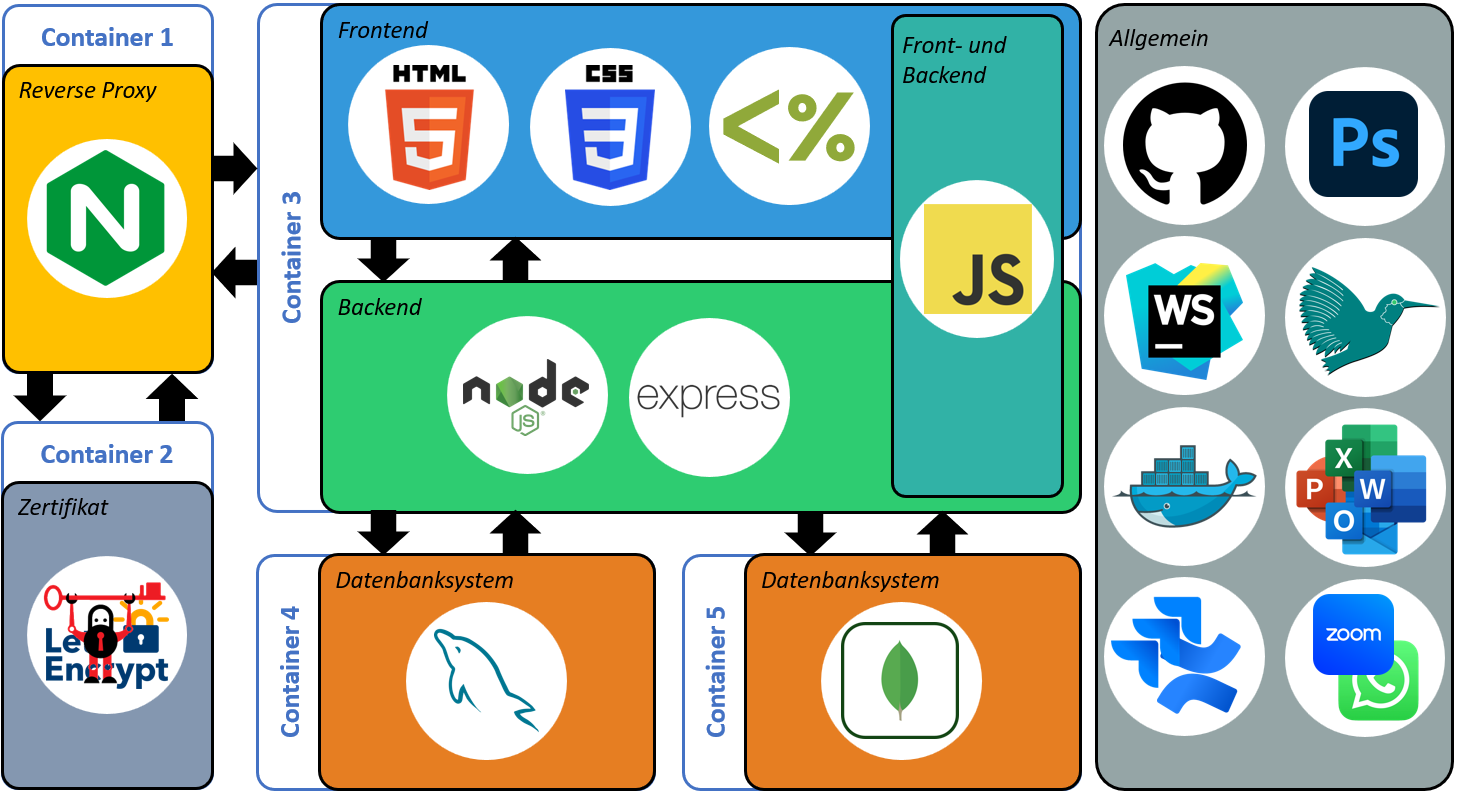
\includegraphics[width=1.0\textwidth]{tools}
    \caption{Übersicht der Tools}\label{fig:uebersicht-tools}
\end{figure}

\subsection{Arbeit mit Pull Requests und Restrictions in Git}\label{subsec:arbeit-mit-pull-requests-und-restrictions-in-git}

Im aktuellen Praxismodul III wurde die bereits im vorherigen Semester eingeführte Arbeitsweise mit separaten Feature-Branches weiterentwickelt und professionalisiert.
Während die Nutzung von Branches bereits in Praxismodul II etabliert wurde, lag der Fokus nun darauf, den Entwicklungsprozess durch verbindliche Strukturen und Regeln qualitativ weiter zu verbessern.

Neu eingeführt wurden sogenannte Pull Requests (PRs), über die Änderungen aus einem Feature-Branch nicht mehr direkt, sondern nur nach expliziter Prüfung durch ein Review in den `main`-Branch übernommen werden dürfen.
Dazu wurden feste Reviewer pro Pull Request definiert, die jeweils für die Freigabe verantwortlich sind.
Bei größeren Änderungen wurde gemeinsame Review Sitzungen während Team Meetings durchgeführt.
Zusätzlich wurden Git-Restrictions aktiviert, welche das direkte Pushen in den `main`-Branch unterbinden.
Dadurch ist sichergestellt, dass keine unkontrollierten Änderungen in die stabile Hauptversion gelangen.

Diese Weiterentwicklung der Git-Nutzung brachte folgende Vorteile mit sich:
\begin{itemize}
    \item Durch Reviews und Restrictions wurden potenziell fehlerhafte oder ungetestete Änderungen frühzeitig erkannt.
    \item Gemeinsame Review Sessions haben zu umfangreicherem Wissenstransfer innerhalb des Teams gesorgt.
    \item Die stabile Version im `main`-Branch konnte nicht durch versehen und unsauberes Arbeiten überschrieben werden.
\end{itemize}

Gleichzeitig entstanden aber auch folgende Herausforderungen:
\begin{itemize}
    \item Im Team musste vorerst ein Verständnis über den neuen Workflow geschaffen werden.
    \item Auch für kleinere Änderungen waren nun zusätzliche Review-Schritte notwendig.
\end{itemize}

Allgemein hat die Einführung der neuen Herangehensweise zu einer strukturierten Arbeitsweise geführt.
